
\usetikzlibrary{arrows.meta}
\begin{frame}{quiz Q1}
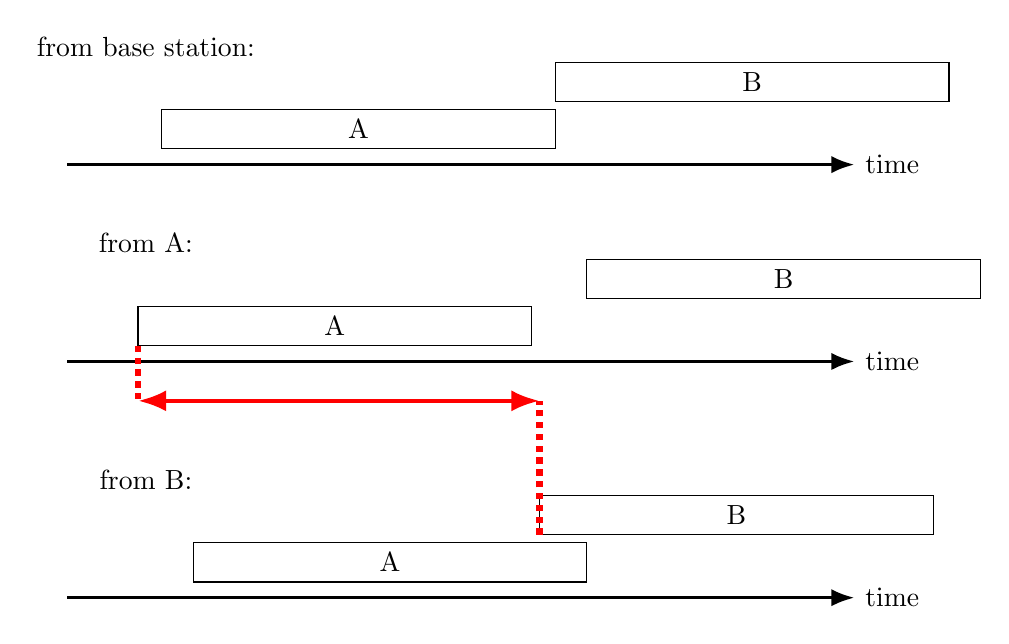
\begin{tikzpicture}
\begin{scope}[]
\node at (0,-.5) {from base station:};
\draw[very thick,-Latex] (-1, -2) -- ++(10, 0) node[right] {time};
\draw (0.2, -1.8) rectangle ++(5, .5) node[midway] {A};
\draw (5.2, -1.2) rectangle ++(5, .5) node[midway] {B};
\end{scope}
\begin{scope}[yshift=-2.5cm]
\node at (0,-.5) {from A:};
\draw[very thick,-Latex] (-1, -2) -- ++(10, 0) node[right] {time};
\draw (-0.1, -1.8) coordinate (real start A) rectangle ++(5, .5) node[midway] {A};
\draw (5.6, -1.2) rectangle ++(5, .5) node[midway] {B};
\end{scope}
\begin{scope}[yshift=-5.5cm]
\node at (0,-.5) {from B:};
\draw[very thick,-Latex] (-1, -2) -- ++(10, 0) node[right] {time};
\draw (0.6, -1.8) rectangle ++(5, .5) node[midway] {A};
\draw (5.0, -1.2) coordinate (real start B) rectangle ++(5, .5) node[midway] {B};
\end{scope}
\coordinate (mid line) at (0, -5);
\draw[ultra thick,red,Latex-Latex] (mid line -| real start A) -- (mid line -| real start B);
\draw[dotted,red,line width=.8mm] (real start A) -- (mid line -| real start A);
\draw[dotted,red,line width=.8mm] (real start B) -- (mid line -| real start B);
\end{tikzpicture}
\end{frame}

